% =========================================================
% CAPÍTULO / SECCIÓN DE MEMORIA — PRÁCTICA 4
% Clasificación y el Valor del Error (Matriz de Costes)
% =========================================================

\section{Práctica 4: Clasificación y el Valor del Error}

\subsection{Objetivo de la práctica}
En esta práctica se entrena un clasificador probabilístico sencillo para un problema de detección de fraude y se analiza cómo el umbral de decisión afecta a los errores y al coste total. El objetivo no es únicamente medir el rendimiento predictivo del modelo, sino estudiar el impacto real de sus decisiones a partir de una matriz de costes.

\subsection{Descripción del problema}
Se trabaja con un problema de clasificación binaria:
\begin{itemize}
  \item \textbf{Clase 0}: transacción normal.
  \item \textbf{Clase 1}: transacción fraudulenta.
\end{itemize}

En este contexto, los errores no tienen el mismo coste:
\begin{itemize}
  \item \textbf{Falso Negativo (FN)}: no detectar un fraude \(\rightarrow 200\,€\)
  \item \textbf{Falso Positivo (FP)}: bloquear una transacción legítima \(\rightarrow 10\,€\)
\end{itemize}

Por tanto, la decisión final no debe evaluarse solo por el número de aciertos, sino por el coste económico asociado a los errores.

% ---------------------------------------------------------
\subsection{Tarea 1: Análisis con el umbral por defecto (\(\tau = 0.5\))}
% ---------------------------------------------------------

\subsubsection{Modelo utilizado}
En esta práctica se ha utilizado una \textbf{Regresión Logística} como clasificador base. El modelo se ha entrenado con el conjunto de entrenamiento y se ha evaluado sobre el conjunto de prueba.

\subsubsection{Matriz de confusión}
A continuación se muestra la matriz de confusión obtenida usando el umbral estándar \(\tau = 0.5\).

\begin{figure}[H]
  \centering
  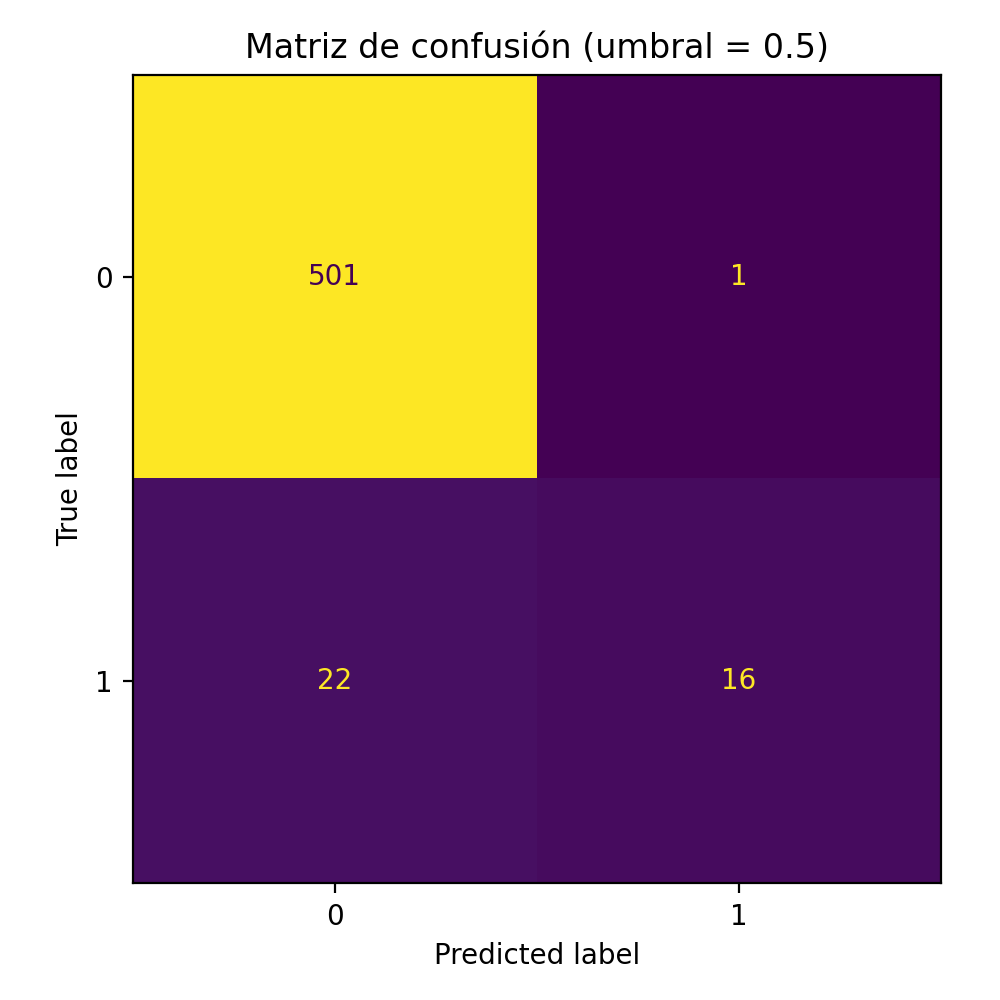
\includegraphics[width=0.48\textwidth]{img/matriz_confusion_umbral_0_5.png}
  \caption{Matriz de confusión para el umbral \(\tau = 0.5\).}
  \label{fig:mc_05}
\end{figure}

A partir de esta matriz, se obtienen los siguientes valores:
\begin{itemize}
  \item Verdaderos Positivos (TP): 16
  \item Verdaderos Negativos (TN): 501
  \item Falsos Positivos (FP): 1
  \item Falsos Negativos (FN): 22
\end{itemize}

\subsubsection{Cálculo del coste total}
El coste total se calcula mediante la expresión:
\[
  \text{Coste Total} = (FP \cdot 10) + (FN \cdot 200)
\]

Sustituyendo los valores obtenidos:
\[
  \text{Coste Total} = (1 \cdot 10) + (22 \cdot 200) = 4410 \,€
\]

\subsubsection{Interpretación}
\textbf{Comentario del alumno:}
\textit{El umbral por defecto de 0.5 no parece en absoluto razonable en este contexto. Si bien el modelo comete pocos falsos positivos (solo 1), está dejando pasar 22 transacciones fraudulentas (falsos negativos). Dado que el coste de no detectar un fraude (200\,€) es veinte veces superior al coste de bloquear una transacción legítima (10\,€), el impacto económico de usar este umbral es muy elevado (4410\,€ en este conjunto). En un entorno real de detección de fraude, un sistema no debe evaluarse solo por la exactitud global si los errores son asimétricos; es fundamental minimizar los errores catastróficos. Por tanto, no usaría este umbral en producción.}

% ---------------------------------------------------------
\subsection{Tarea 2: Estudio de probabilidades y umbrales}
% ---------------------------------------------------------

\subsubsection{Análisis de distintos umbrales}
En lugar de trabajar únicamente con la clase predicha, se han utilizado las probabilidades estimadas por el modelo para la clase positiva y se han evaluado distintos valores del umbral \(\tau\) entre 0 y 1, en pasos de 0.05.

La Tabla~\ref{tab:umbrales_coste} resume los resultados obtenidos para varios umbrales.

\begin{table}[H]
  \centering
  \caption{Resumen de resultados para distintos umbrales.}
  \label{tab:umbrales_coste}
  \begin{tabular}{c c c c}
    \toprule
    \textbf{Umbral} & \textbf{FP} & \textbf{FN} & \textbf{Coste Total (€)} \\
    \midrule
    0.00            & 502         & 0           & 5020                     \\
    0.05            & 112         & 9           & 2920                     \\
    0.10            & 42          & 14          & 3220                     \\
    0.15            & 22          & 15          & 3220                     \\
    0.20            & 13          & 15          & 3130                     \\
    \vdots          & \vdots      & \vdots      & \vdots                   \\
    1.00            & 0           & 38          & 7600                     \\
    \bottomrule
  \end{tabular}
\end{table}

\subsubsection{Observaciones}
\textbf{Comentario del alumno:}
\textit{Existe un claro compromiso o ``trade-off'' entre ambos tipos de error al variar el umbral de decisión. Cuando el umbral baja (hacia 0), exigimos menos confianza para clasificar una observación como fraude. En consecuencia, capturamos más transacciones fraudulentas reduciendo drásticamente los Falsos Negativos (con umbral de 0 bajamos a 0 FN), pero al mismo tiempo generamos muchos Falsos Positivos (bloqueamos transacciones normales equivocadamente).
  Por otro lado, cuando el umbral sube (hacia 1), nos volvemos tan exigentes que apenas saltan alarmas, los Falsos Positivos se reducen considerablemente (con umbral 1.0 hay 0 FP), pero se nos escapan masivamente los casos fraudulentos reales (aumentan los Falsos Negativos). }

% ---------------------------------------------------------
\subsection{Tarea 3: Optimización del coste}
% ---------------------------------------------------------

\subsubsection{Gráfica de coste frente a umbral}
La Figura~\ref{fig:coste_umbral} muestra la evolución del coste total en función del umbral de decisión.

\begin{figure}[H]
  \centering
  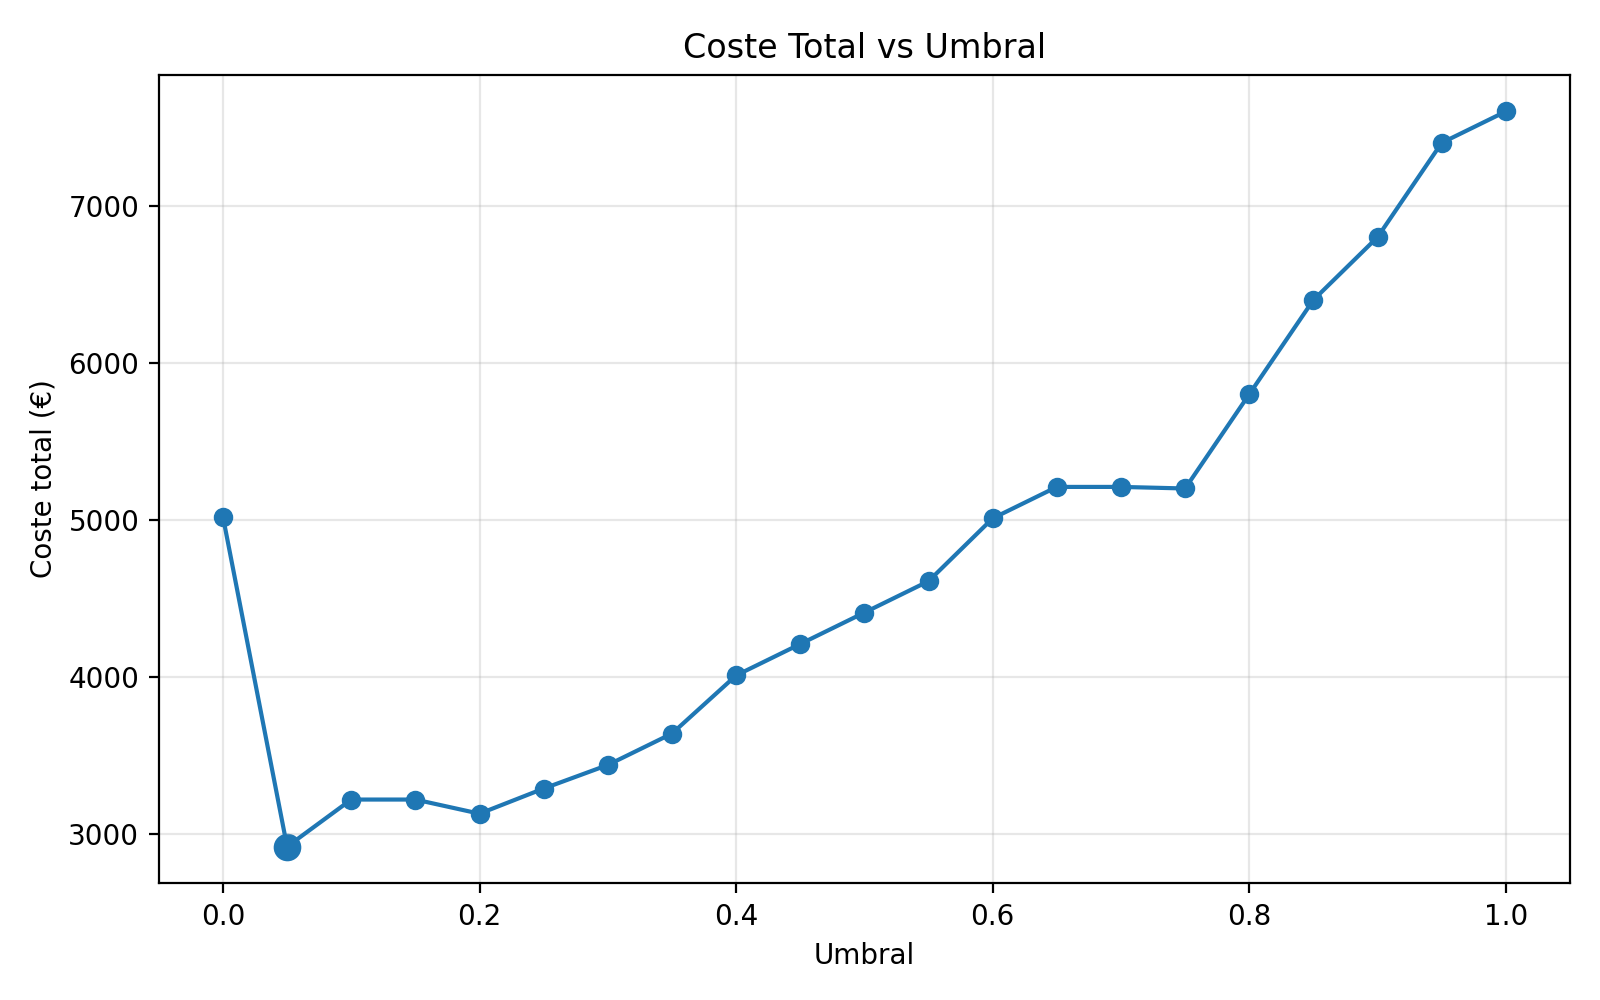
\includegraphics[width=0.72\textwidth]{img/coste_vs_umbral.png}
  \caption{Coste total en función del umbral de decisión.}
  \label{fig:coste_umbral}
\end{figure}

\subsubsection{Umbral óptimo}
A partir de la gráfica y de la tabla anterior, el umbral que minimiza el coste total es:

\[
  \tau^* = 0.05
\]

El coste total mínimo asociado es:

\[
  \text{Coste mínimo} = 2920 \,€
\]

\subsubsection{Interpretación}
\textbf{Comentario del alumno:}
\textit{El umbral óptimo (\(\tau^* = 0.05\)) es muy inferior a 0.5. Esto tiene todo el sentido en el contexto del problema, dada la fuerte penalización por pasar por alto un fraude; el coste de un falso negativo (200\,€) es veinte veces el de un falso positivo (10\,€). Al inclinar la matriz hacia penalizaciones asimétricas, el punto de coste mínimo se desplaza rápidamente para favorecer al error más 'barato' a expensas de tolerar una mayor cantidad del mismo. Para el banco es mucho más razonable adoptar una estrategia «conservadora»: es preferible molestar interrumpiendo algunas cuentas sanas a permitir que se consumen cuantiosos fraudes sin ser bloqueados.}

% ---------------------------------------------------------
\subsection{Tarea 4: Curvas ROC y Precision-Recall}
% ---------------------------------------------------------

\subsubsection{Curva ROC}
La Figura~\ref{fig:roc} muestra la curva ROC obtenida para el modelo.

\begin{figure}[H]
  \centering
  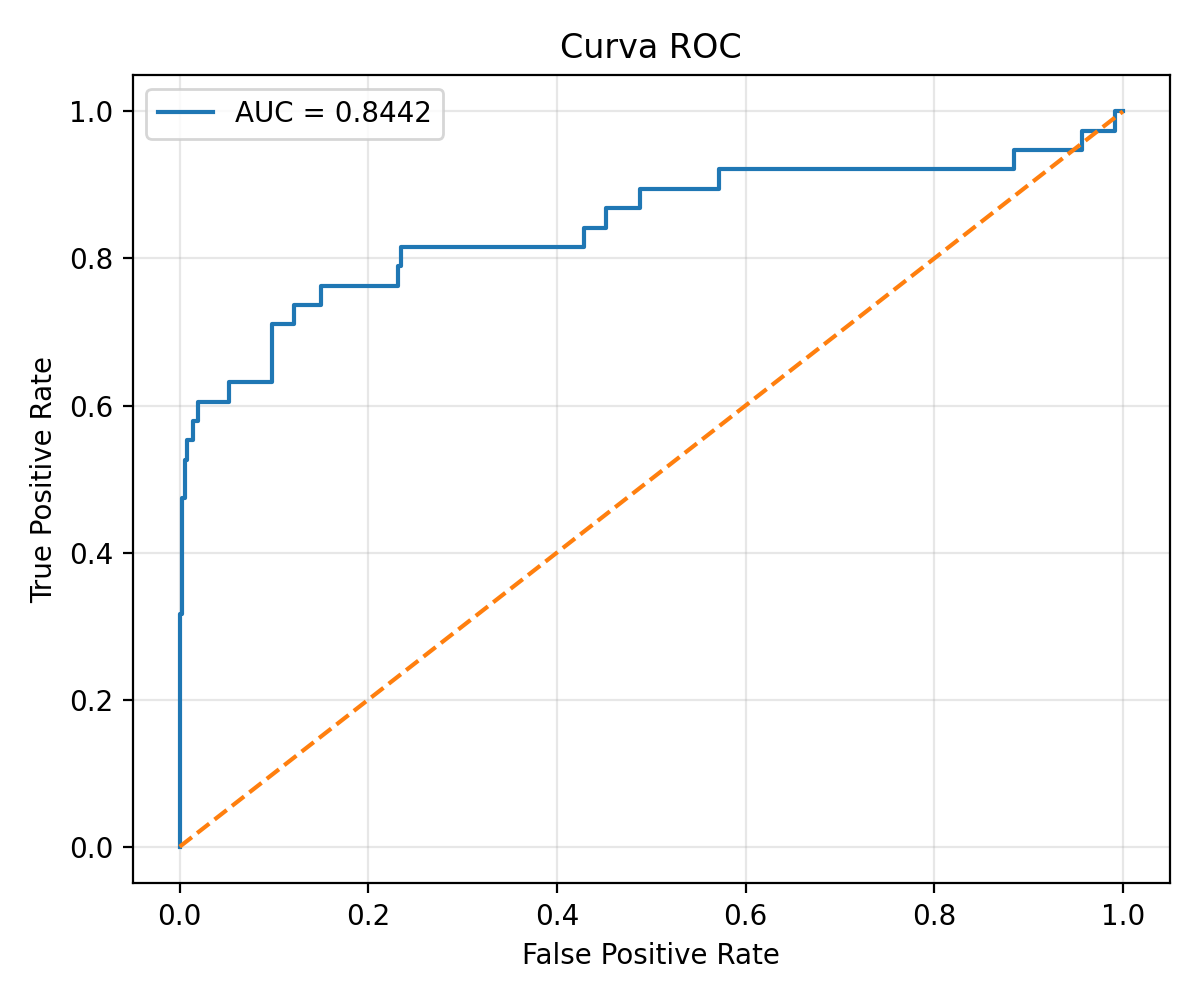
\includegraphics[width=0.58\textwidth]{img/curva_roc.png}
  \caption{Curva ROC del clasificador.}
  \label{fig:roc}
\end{figure}

\subsubsection{Curva Precision-Recall}
La Figura~\ref{fig:pr} muestra la curva Precision-Recall del modelo.

\begin{figure}[H]
  \centering
  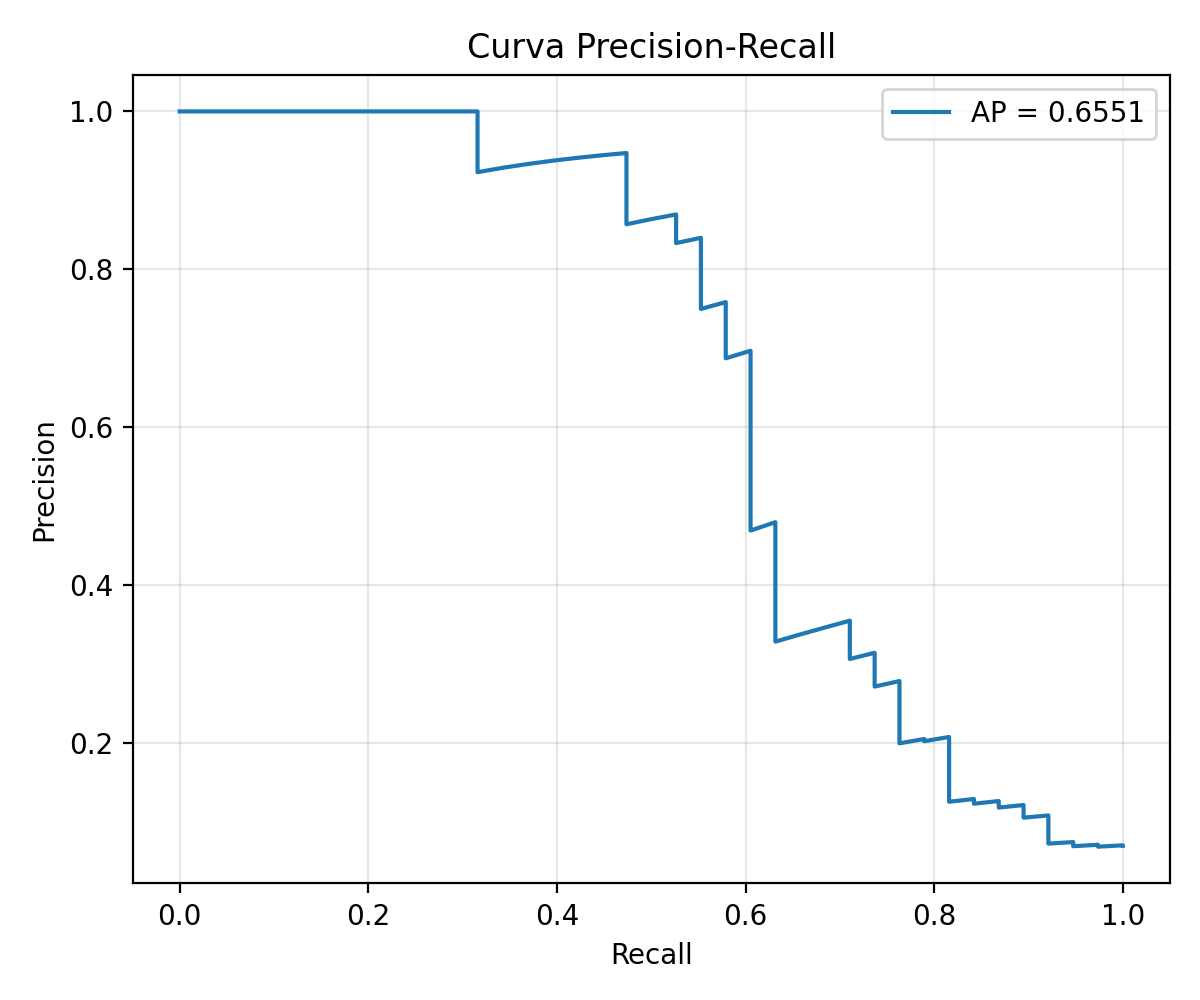
\includegraphics[width=0.58\textwidth]{img/curva_precision_recall.png}
  \caption{Curva Precision-Recall del clasificador.}
  \label{fig:pr}
\end{figure}

\subsubsection{Discusión}
\textbf{Comentario del alumno:}
\textit{En este problema donde el dataset es presumiblemente desbalanceado (pocos fraudes en comparación con un abrumador volumen de transacciones normales), la Curva Precision-Recall (PR) es más informativa. La curva ROC puede resultar engañosa porque considera el False Positive Rate (FPR), que utiliza en su denominador el inmenso total de transacciones negativas. Cuando la clase mayoritaria es gigantesca, un pequeño incremento en Falsos Positivos casi no mueve el ratio de FPR y mantiene el AUC-ROC artificialmente alto. Sin embargo, en la gráfica de Precisión vs Recall observamos cómo las alertas dadas como positivas reflejan en realidad muchísimos Falsos Positivos en la base Precision (TP / (TP + FP)); por ende el impacto del aumento de errores sí se percibe mejor. En el departamento de seguridad interesa especialmente esta curva (PR) para observar cuán preciso eres al recuperar esta clase minoritaria de intrusiones y fraudes.}

% ---------------------------------------------------------
\subsection{Decisión final de ingeniería}
% ---------------------------------------------------------

Imaginando que formo parte del equipo técnico del banco, la política de decisión que recomendaría sería la siguiente:

\begin{quote}
  Recomiendo de forma concluyente apartarnos del umbral por defecto (0.5) y bajar el umbral de decisión a $\tau = 0.05$. Con esto pasamos de los $4410$€ de coste a un mínimo evaluado de $2920$€. Es cierto que esta bajada radical incrementa significativamente el número de Falsos Positivos, pero el fraude económico tiene tal impacto que la prioridad debe ser detectarlo a tiempo (minimizando los Falsos Negativos a toda costa). El usuario legítimo que sufra un bloqueo falso, sentirá una ligera molestia, que el banco puede absorber con un coste inferior mediante alertas por SMS de desbloqueo rápido al teléfono, mientras que el perjuicio del fraude masivo es un golpe directo y devastador a la contabilidad de la entidad (un coste 20x).
\end{quote}

\noindent Esta decisión se basa en:
\begin{itemize}
  \item el coste asociado a los falsos positivos y falsos negativos;
  \item el umbral que minimiza el coste total económico;
  \item el equilibrio entre seguridad operativa contra el riesgo financiero y molestias puntuales para el cliente;
  \item la fuerte caída de precisión real vista en la curva Precision-Recall.
\end{itemize}

% ---------------------------------------------------------
\subsection{Conclusiones}
% ---------------------------------------------------------

\textbf{Comentario final del alumno:}
\textit{Con esta práctica he aprendido un concepto muy valioso: el mejor modelo estadístico en abstracto no es el mejor modelo en producción, a menos que esté calibrado para el caso de negocio al que se aplica. Especialmente cuando abordamos problemas desestructurados o asimétricos, los errores no tienen un impacto plano (no "valen lo mismo"): en contextos de salud, seguridad, y monitorización financiera es mandatorio usar o bien matrices condicionales de coste económico en lugar de baremos ingenuos o simétricos. Variando el umbral se regula directamente la sensibilidad hacia un error en concreto. Ninguna métrica como el \emph{Accuracy} sirve frente al desbalance; una evaluación seria tiene siempre que incorporar el contexto experto del dominio e informar las decisiones en parámetros que prioricen la minimización genuina del riesgo y perjuicio material.}